\chapter{Les Tableaux de Bord}\label{chap:tableaux-de-bord}
\index{les tableaux de bord}

\utilisateurs: \lienmanager.\\

\chapintro{Ce chapitre d\'ecrit comment consulter les
		 	tableaux de bord. En effet, bon nombre de
		 	d\'ecisions des \manager proviennent de la
		 	visualisation des rapports financiers, et
		 	commerciaux.}

\nxsection{Introduction}\label{sec:tableaux-introduction}

\begin{figure}[!htbp]
	\centering
	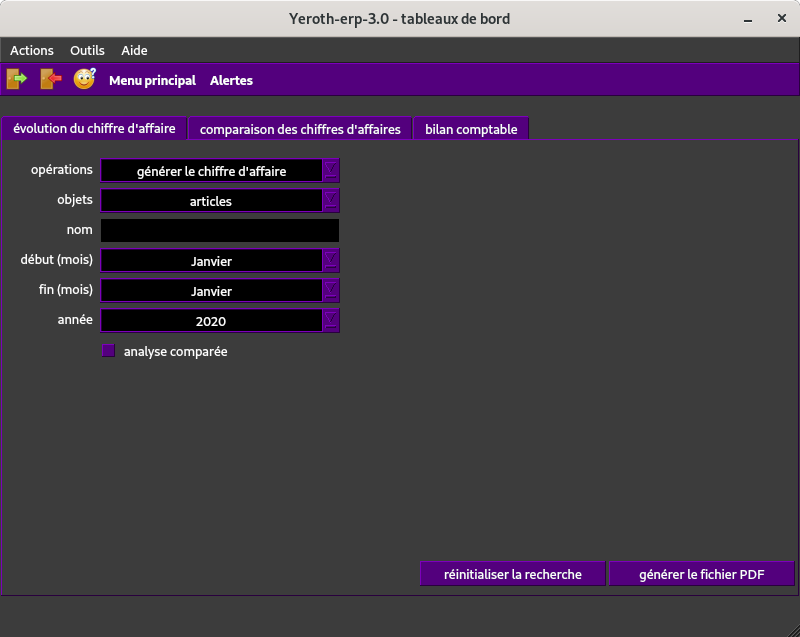
\includegraphics[scale=0.45]{images/yeren-rapports.png}
	\caption{La fen\^etre principale pour g\'en\'erer les rapports commerciaux.}
	\label{fig:yeroth-tableaux}
\end{figure}

La figure~\ref{fig:yeren-rapports} illustre l'interface
de \yeren pour param\'etrer et g\'en\'erer l'\'evolution
du chiffre d'affaire (au format PDF) sur une p\'eriode de temps.

L'interface graphique 'comparaison des chiffres d'affaires'
(figure~\ref{fig:yeren-rapports-comparaison-articles})
permet \`a l'utilisateur de comparer les chiffres
d'affaire d'objets allant de $2$ \`a $9$ unit\'es.

Les objets de comparaisons sont les suivants:
\begin{enumerate}[1)]
	\item le chiffre d'affaire des articles vendus
	\item le chiffre d'affaire des cat\'egories d'articles vendues
	\item le chiffre d'affaire des clients nomm\'es de l'entreprise
	\item le chiffre d'affaire des caissiers de l'entreprise.\\
\end{enumerate}

L'utilisateur a le choix entre les diagrammes comparatifs
suivants:
\begin{enumerate}[1)]
	\item le diagramme en bande
	\item le diagramme circulaire.\\
\end{enumerate}

La figure~\ref{fig:diagramme-bande-chiffre-daffaire-comparatif-articles}
et~\ref{fig:diagramme-circulaire-chiffre-daffaire-comparatif-articles}
illustrent des examples de diagramme comparatif en 'diagramme en bande'
et en 'diagramme circulaire' respectivement.

\nxsection{G\'en\'erer l'\'evolution du chiffre
			d'affaire}\label{sec:evolution-chiffre-affaire}
\index{g\'en\'erer l'\'evolution du chiffre d'affaire}
\index{\'evolution du chiffre d'affaire}

Il faut effectuer les actions suivantes dans l'interface
graphique de \yeren illustr\'ee dans la
figure~\ref{fig:yeren-rapports}:

\begin{enumerate}[1)]
	\item choisir la date de 'd\'ebut (mois)'
	\item choisir la date de 'fin (mois)'	
	\item choisir l'ann\'ee souhait\'ee
	\item conclure an cliquant dur le
		bouton \bouton{g\'en\'erer le fichier PDF}.
\end{enumerate}

%-----------------------------------------------------------
\newpage
\nxsection{G\'en\'erer les chiffres d'affaires de plusieurs
	articles de fa\c{c}on comparative
	}\label{sec:comparaison-chiffre-affaire-articles}
\index{g\'en\'erer les chiffres d'affaires de plusieurs	articles de fa\c{c}on comparative}
\index{comparer les chiffres d'affaires de plusieurs articles}

La figure~\ref{fig:yeren-rapports-comparaison-articles}
illustre comment g\'en\'erer un diagramme en bande,
comparatif des quatre articles avec les chiffres d'affaires
les plus \'elev\'es.\\

\begin{figure}[!htbp]
	\centering
	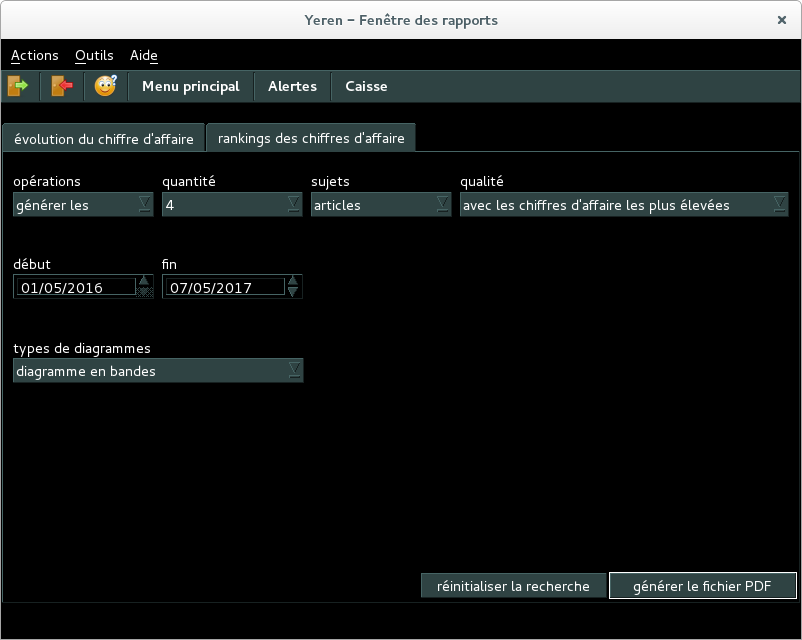
\includegraphics[scale=0.45]{images/yeren-rapports-comparaison-articles.png}
	\caption{Une figure comparative des chiffres d'affaires de
		quatre articles de la fen\^etre des rapports commerciaux.}
	\label{fig:yeroth-tableaux-comparaison-articles}
\end{figure}

La figure~\ref{fig:diagramme-bande-chiffre-daffaire-comparatif-articles}
illustre le fichier PDF g\'en\'er\'e avec pour option 'diagramme en bandes'.

%\newpage

\begin{figure}[!htbp]
	\centering
	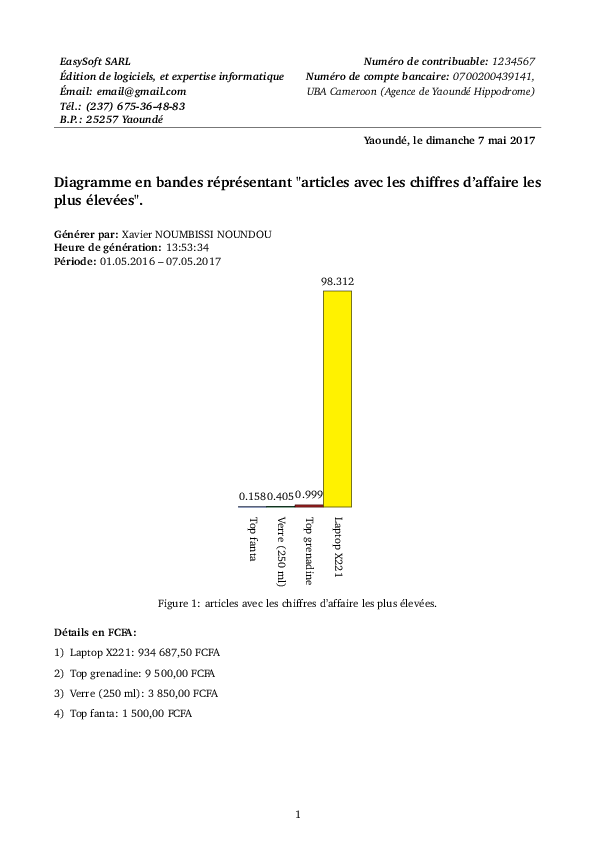
\includegraphics[scale=0.65]{images/diagramme-bande-chiffre-daffaire-comparatif-articles.png}
	\caption{Une figure comparative du chiffre d'affaire de
		quatre articles \`a l'aide d'un digramme en bande.}
	\label{fig:diagramme-bande-chiffre-daffaire-comparatif-articles}
\end{figure}

La figure~\ref{fig:diagramme-circulaire-chiffre-daffaire-comparatif-articles}
illustre le fichier PDF g\'en\'er\'e avec pour option 'diagramme circulaire'.

\begin{figure}[!htbp]
	\centering
	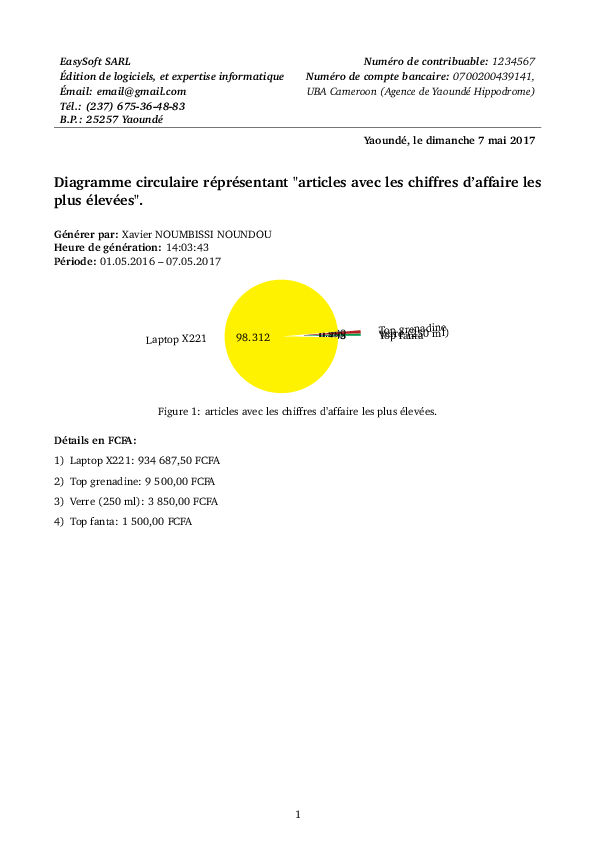
\includegraphics[scale=0.65]{images/diagramme-circulaire-chiffre-daffaire-comparatif-articles.png}
	\caption{Une figure comparative du chiffre d'affaires de
		quatre articles \`a l'aide d'un digramme circulaire.}
	\label{fig:diagramme-circulaire-chiffre-daffaire-comparatif-articles}
\end{figure}

%-----------------------------------------------------------

\newpage
\nxsection{G\'en\'erer les chiffres d'affaires de plusieurs
			cat\'egories articles de fa\c{c}on comparative}
\index{g\'en\'erer les chiffres d'affaires de plusieurs
		cat\'egories articles de fa\c{c}on comparative}

Il faut proc\'eder comme \`a la section~\ref{sec:comparaison-chiffre-affaire-articles}, juste
en changeant le combo box '\textbf{sujets}' d'articles \`a
'\textbf{cat\'egories}' et le combo box '\textbf{qualit\'e}'.

%-----------------------------------------------------------

\nxsection{G\'en\'erer les chiffres d'affaires de plusieurs
			clients de fa\c{c}on comparative}
\index{g\'en\'erer les chiffres d'affaires de plusieurs 
		clients de fa\c{c}on comparative}

Il faut proc\'eder comme \`a la section~\ref{sec:comparaison-chiffre-affaire-articles}, juste
en changeant le combo box '\textbf{sujets}' d'articles \`a
'\textbf{clients}' et le combo box '\textbf{qualit\'e}'.

%-----------------------------------------------------------

\nxsection{G\'en\'erer les chiffres d'affaires de plusieurs
			caissiers de fa\c{c}on comparative}
\index{g\'en\'erer les chiffres d'affaires de plusieurs
		caissiers de fa\c{c}on comparative}

Il faut proc\'eder comme \`a la section~\ref{sec:comparaison-chiffre-affaire-articles}, juste
en changeant le combo box '\textbf{sujets}' d'articles \`a
'\textbf{caissiers}' et le combo box '\textbf{qualit\'e}'.

